\documentclass[12pt,a4paper]{article}

% --- Encoding & Language ---
\usepackage[utf8]{inputenc}
\usepackage[T1]{fontenc}
\usepackage[brazil]{babel}

% --- Layout ---
\usepackage[a4paper, top=3cm, bottom=2cm, left=3cm, right=2cm]{geometry}
\usepackage{indentfirst}
\usepackage{setspace}
\onehalfspacing

% --- Graphics & Floats ---
\usepackage{graphicx}
\usepackage{float}

% --- Links ---
\usepackage[hidelinks]{hyperref}

% --- Tables ---
\usepackage{booktabs}
\usepackage{longtable}
\usepackage{array}
\usepackage{multirow}
\usepackage{xcolor}
\usepackage{colortbl}
\usepackage{tabularx}
\newcommand{\lightrule}{\arrayrulecolor{gray!35}\midrule\arrayrulecolor{black}}

% --- Code ---
\usepackage{listings}
\definecolor{backcolour}{rgb}{0.95,0.95,0.92}
\definecolor{codegreen}{rgb}{0,0.5,0}
\lstdefinestyle{codestyle}{
    backgroundcolor=\color{backcolour},
    commentstyle=\color{codegreen}\itshape,
    keywordstyle=\color{blue}\bfseries,
    basicstyle=\ttfamily\footnotesize,
    breaklines=true,
    keepspaces=true,
    numbers=left,
    numberstyle=\tiny\color{gray},
    numbersep=5pt,
    tabsize=2,
    frame=single,
    rulecolor=\color{gray!40}
}
\lstset{style=codestyle}

% --- Lists ---
\usepackage{enumitem}

% --- Status helpers ---
\newcommand{\aprovado}{\textcolor{green!60!black}{\textbf{Aprovado}}}
\newcommand{\parcial}{\textcolor{orange!80!black}{\textbf{Parcialmente Testado}}}
\newcommand{\naorealizado}{\textcolor{gray}{\textbf{Não Realizado}}}
\newcommand{\reprovado}{\textcolor{red}{\textbf{Reprovado}}}

% =========================================================
\begin{document}

% =========================================================
% CAPA
% =========================================================
\begin{titlepage}
    \centering
    \vspace*{1.5cm}

    {\large\bfseries Universidade Federal de Minas Gerais}\\[0.3cm]
    {\large Escola de Engenharia}\\[0.3cm]
    {\large Laboratório de Sistemas I --- PLSI}\\[0.2cm]
    {\large Prof. Diogo Batista de Oliveira}\\

    \vspace{3cm}

    {\Huge\bfseries PillHub}\\[0.5cm]
    {\Large Sistema Automatizado de Dispensação de Medicamentos}

    \vspace{2cm}

    {\large Relatório Final}

    \vspace{2.5cm}

    \begin{tabular}{l}
        Felippe Veloso Marinho    \\[0.2cm]
        Igor Braga de Lima        \\[0.2cm]
        Josoé Santos Queiroz      \\[0.2cm]
        Luiz Daniel de Lima Pião  \\[0.2cm]
        Raissa Gonçalves Diniz    \\
    \end{tabular}

    \vfill

    {\large Belo Horizonte, junho de 2026}
\end{titlepage}

% =========================================================
% SUMÁRIO
% =========================================================
\tableofcontents
\newpage

% =========================================================
% RESUMO
% =========================================================
\section*{Resumo}
\addcontentsline{toc}{section}{Resumo}

O Dispenser Inteligente é um sistema embarcado de dispensação automática de medicamentos desenvolvido para promover a autonomia e a segurança de pacientes atendidos por um centro de reabilitação. O sistema é composto por um dispositivo físico baseado no microcontrolador ESP32-C3, um servidor de backend em FastAPI (Python) com banco de dados PostgreSQL, e um painel de controle web em React. O dispenser realiza a liberação de comprimidos em horários programados, emite alertas multimodais (sonoro, visual e vibratório) e registra a confirmação do paciente. Este relatório descreve a arquitetura do sistema, as decisões de implementação, a validação dos requisitos por meio de casos de teste e uma análise crítica do processo de desenvolvimento segundo o modelo cascata.

\newpage

% =========================================================
% 1. INTRODUÇÃO
% =========================================================
\section{Introdução}

\subsection{Contexto}

O Centro de Reabilitação objeto deste projeto (Centro de Reabilitação Rames Ossen Ali, em Igrarapé) atende pacientes encaminhados por unidades básicas de saúde para serviços de fisioterapia, terapia ocupacional e fonoaudiologia. O perfil dos pacientes é heterogêneo: incluem pessoas com Transtorno do Espectro Autista (TEA), Transtorno do Déficit de Atenção e Hiperatividade (TDAH), deficiências físicas e sensoriais (visuais e auditivas), membros amputados, e sequelas neurológicas como acidente vascular cerebral (AVC) e paralisia cerebral, abrangendo todas as faixas etárias, de bebês a idosos.

O centro não administra medicamentos em suas instalações. Os pacientes e seus cuidadores são responsáveis pelo regime medicamentoso em casa, o que cria desafios significativos: esquecimento de doses, erros de horário, dificuldade de manipulação de embalagens convencionais e ausência de feedback ao cuidador em caso de não adesão.

\subsection{Problema}

O principal problema identificado é a \textbf{falta de adesão ao regime medicamentoso domiciliar} por parte de pacientes com comprometimentos cognitivos, motores ou sensoriais. Para pacientes com TEA e TDAH, a rigidez de rotina e a dificuldade de lidar com alertas invasivos tornam o problema ainda mais crítico. A não adesão à medicação é uma das principais causas de internação evitável e piora de quadros clínicos crônicos.

\subsection{Objetivos}

\textbf{Objetivo geral:} Desenvolver um sistema integrado de dispensação automática de medicamentos que promova a autonomia, a segurança e a qualidade de vida de pacientes com necessidades especiais.

\textbf{Objetivos específicos:}
\begin{itemize}
    \item Implementar um mecanismo físico de dispensação controlada por software;
    \item Criar um sistema de alertas multimodal acessível (sonoro, visual e vibratório) com modo silencioso;
    \item Desenvolver uma interface web de configuração de horários e monitoramento;
    \item Garantir notificação ao cuidador em caso de não confirmação pelo paciente;
    \item Registrar histórico de adesão para acompanhamento clínico.
\end{itemize}

\newpage

% =========================================================
% 2. DESCRIÇÃO DO SISTEMA
% =========================================================
\section{Descrição do Sistema}

\subsection{Visão Geral}

O Dispenser Inteligente é um dispositivo de mesa composto por uma roleta com 30 compartimentos individuais, cada um destinado a armazenar a medicação de uma dispensação específica (três dispensações diárias por dez dias). O dispositivo deve ser regularmente reabastecido pelo cuidador e opera de forma autônoma, liberando o compartimento correto nos horários pré-configurados e emitindo alertas para que o paciente confirme a retirada.

O sistema é dividido em quatro camadas funcionais:

\begin{enumerate}
    \item \textbf{Hardware/Firmware:} o dispositivo físico com o microcontrolador, motor, sensores e atuadores;
    \item \textbf{Backend:} servidor de API responsável pela lógica de negócio, agendamentos e proxy para o hardware;
    \item \textbf{Frontend:} painel web para configuração, monitoramento e histórico;
    \item \textbf{Banco de dados:} persistência de pacientes, medicamentos, agendas e registros de dispensação.
\end{enumerate}

\subsection{Público-Alvo e Contexto de Uso}

O sistema é destinado a uso \textbf{exclusivamente residencial}. O paciente interage com o dispositivo físico para confirmar a retirada do medicamento. O cuidador (familiar, enfermeiro domiciliar ou terapeuta) configura o sistema pelo painel web e recebe notificações (vai e-mail) caso o paciente não responda dentro do prazo definido (atualmente 2 minutos, mas é um parâmetro configurável, se na prática um período maior for necessário).

A diversidade do público-alvo também impôs alguns requisitos de acessibilidade: alertas não agressivos para pacientes com algum tipo de sensibilidade sensorial, LEDs de alta luminosidade com simbologia de período do dia (sol para manhã, sol com nuvem para tarde, lua para noite), botão físico de confirmação grande e de fácil acionamento, e interface visual com baixa carga cognitiva.

\subsection{Funcionalidades Principais}

\begin{itemize}
    \item \textbf{Dispensação automática:} liberação do slot correto no horário programado, sem manipulação manual pelo paciente;
    \item \textbf{Rastreamento de confirmação:} o dispositivo expõe o flag \texttt{awaiting\_confirm} no \texttt{GET /status}, sinalizando ao backend quando uma dispensação está pendente de confirmação. O backend pode (e deve) verificar esse estado antes de acionar uma nova dispensação para evitar doses duplicadas;
    \item \textbf{Alertas multimodais simultâneos:}
        \begin{itemize}
            \item Sonoro: buzzer (modo normal);
            \item Visual: LED vermelho para manhã (GPIO 7), LED amarelo para tarde (GPIO 1), LED verde para noite (GPIO 0);
            \item Vibratório: micro motor de vibração em modo silencioso;
        \end{itemize}
    %\item \textbf{Persistência dos alertas} até confirmação do paciente;
    \item \textbf{Confirmação pelo paciente:} botão físico (GPIO 3) ou confirmação remota via API;
    \item \textbf{Notificação ao cuidador:} caso o paciente não confirme em tempo determinado;
    \item \textbf{Registro de histórico:} cada dispensação e confirmação é registrada para acompanhamento de adesão;
    \item \textbf{Modo reabastecimento:} permite ao cuidador acessar os compartimentos sem acionar a lógica de dispensação. Ao ativar o modo pelo painel web, o firmware passa a bloquear qualquer comando de dispensação até que o cuidador clique em ``Concluir reabastecimento e iniciar ciclo'', que calibra a roleta e retoma a operação normal;
    \item \textbf{Modo de demonstração:} sequência automatizada de dispensação nos três períodos (manhã → tarde → noite) com intervalo de 30~s entre cada etapa, permitindo ao cuidador verificar o funcionamento completo do hardware sem aguardar agendamentos reais.
\end{itemize}

\subsection{Componentes de Hardware}

\begin{table}[H]
    \centering
    \caption{Componentes de hardware do Dispenser}
    \label{tab:hardware}
    \begin{tabularx}{\textwidth}{lXl}
        \toprule
        \textbf{Componente}   & \textbf{Especificação}                & \textbf{Peça} \\
        \lightrule
        Microcontrolador      & WiFi, 3--5V, programável              & ESP32-C3 SuperMini \\
        \lightrule
        Motor de passo        & Girar 1 slot por vez, 5V              & Micro Servomotor SG90 \\
        \lightrule
        Alerta sonoro         & Mínimo 60 dB, 5V                      & Buzzer Ativo 5V \\
        \lightrule
        Alerta vibratório     & Silencioso, estrutura segura          & Micro Motor 3V \\
        \lightrule
        Alerta visual         & Alta luminosidade, 3 períodos         & 3$\times$ LED 5mm \\
        \lightrule
        Botão confirmação     & Tátil, grande, GPIO 3                 & Push Button 12$\times$12mm \\
        \lightrule
        Alimentação           & 127V, até 1A                          & Carregador USB padrão \\
        \bottomrule
    \end{tabularx}
\end{table}

\subsection{Casos de Uso}

Os casos de uso do sistema, levantados durante a fase de modelagem, são:

\begin{enumerate}
    \item Configurar horários de dispensação via painel web;
    \item Receber alerta de dispensação (sonoro, visual ou vibratório);
    \item Confirmar tomada de medicamento (botão físico);
    \item Reabastecer o dispenser (modo reabastecimento);
    \item Receber notificação de não adesão (cuidador);
    \item Registrar dose no histórico;
    \item Visualizar histórico de adesão.
\end{enumerate}

% =========================================================
% 3. ARQUITETURA DO SISTEMA
% =========================================================
\section{Arquitetura do Sistema}

\subsection{Visão em Camadas}

\begin{figure}[H]
\centering
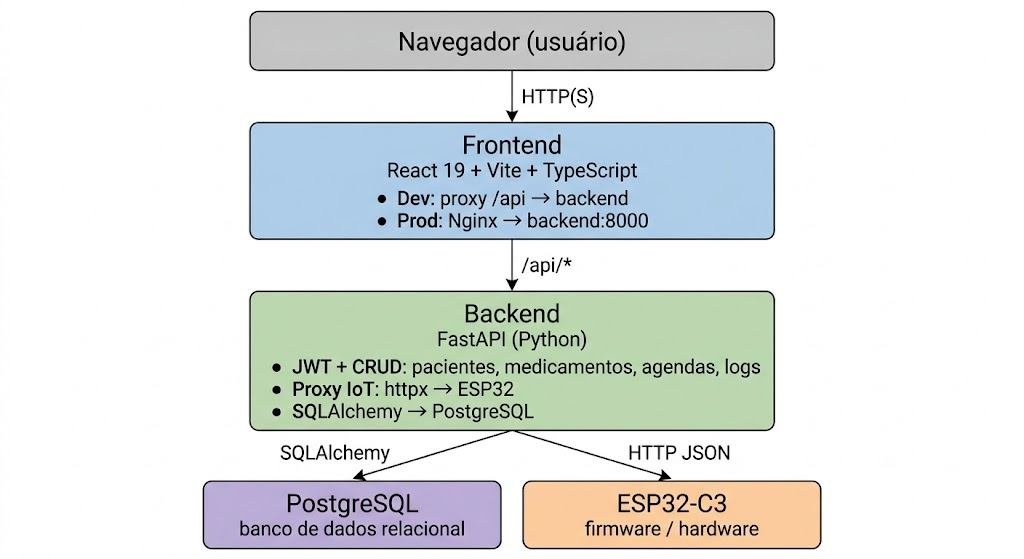
\includegraphics[width=0.85\textwidth]{arquitetura.png}
\caption{Arquitetura em camadas do Dispenser}
\label{fig:arquitetura}
\end{figure}

\subsection{Descrição dos Módulos}

\textbf{Firmware (ESP32-C3):} servidor HTTP assíncrono rodando diretamente no microcontrolador. Expõe uma API REST que o backend consome para acionar o hardware e consultar o estado do dispositivo. Opera em rede WiFi local.

\textbf{Backend (FastAPI):} servidor Python que atua como intermediário entre o frontend e o hardware. Gerencia autenticação JWT, persiste dados de pacientes, medicamentos, agendamentos e logs, e faz proxy de requisições IoT para o firmware via cliente HTTP assíncrono (\texttt{httpx}).

\textbf{Frontend (React):} painel web responsivo para configuração de horários, monitoramento em tempo real do estado do dispenser e visualização do histórico de adesão. Comunica-se exclusivamente com o backend via prefixo \texttt{/api}.

\textbf{Banco de Dados (PostgreSQL):} armazenamento relacional com schema inicializado via \texttt{database/init.sql}. Os modelos são gerenciados pelo SQLAlchemy no backend.

\subsection{Fluxo de Comunicação Típico}

A comunicação entre firmware e backend é baseada em \textbf{heartbeat periódico}: o ESP32 é quem inicia a conexão, eliminando a necessidade de o backend conhecer o IP do dispositivo com antecedência.

\begin{enumerate}
    \item O cuidador acessa o painel web e configura os horários de dispensação (manhã, tarde e noite).
    \item O \textbf{scheduler} do backend (tarefa assíncrona em background) verifica a cada 10 segundos quais agendamentos estão no prazo; ao detectar um, enfileira um comando \texttt{dispense} na tabela \texttt{pending\_commands}.
    \item O firmware envia \texttt{POST /api/heartbeat} ao backend a cada 30 segundos (ou imediatamente após uma confirmação do paciente). O corpo inclui \texttt{current\_slot}, \texttt{awaiting\_confirm}, \texttt{critical\_stock}, RSSI e, se aplicável, o ACK do último comando executado.
    \item O backend responde ao heartbeat com o próximo comando pendente (\texttt{dispense} ou \texttt{calibrate}), marcando-o como entregue. Se não há comando, responde com \texttt{"command": null}.
    \item Ao receber um comando \texttt{dispense}, o firmware avança a roleta (servo SG90), acende o LED do período e dispara o alerta: buzzer em modo normal, ou vibração persistente em pulsos até confirmação no \textbf{modo silencioso}.
    \item O paciente retira o medicamento e pressiona o botão físico de confirmação; o firmware limpa os alertas e agenda um heartbeat imediato para notificar o backend.
    \item O backend recebe o ACK no próximo heartbeat, marca o comando como concluído, atualiza o flag \texttt{awaiting\_confirm} e persiste o evento no log de dispensações.
    \item Se não houver confirmação dentro do prazo, o backend notifica o cuidador por e-mail.
\end{enumerate}

\newpage

% =========================================================
% 4. IMPLEMENTAÇÃO
% =========================================================
\section{Implementação}

\subsection{Firmware (ESP32-C3)}

O firmware foi desenvolvido em C++ utilizando o Arduino IDE com o core ESP32 versão \textbf{2.0.17} (versões 3.x são incompatíveis com as bibliotecas assíncronas utilizadas). As bibliotecas principais são \texttt{ESPAsyncWebServer} e \texttt{AsyncTCP}.

A API HTTP exposta pelo firmware possui os seguintes endpoints:

\begin{table}[H]
    \centering
    \caption{Endpoints da API do firmware}
    \label{tab:endpoints}
    \begin{tabularx}{\textwidth}{llX}
        \toprule
        \textbf{Método} & \textbf{Rota}           & \textbf{Descrição} \\
        \lightrule
        GET             & \texttt{/status}        & Retorna estado completo do dispositivo \\
        \lightrule
        POST            & \texttt{/dispense}      & Avança roleta e dispara alertas \\
        \lightrule
        POST            & \texttt{/confirm}       & Confirma retirada e limpa alertas \\
        \lightrule
        POST            & \texttt{/calibrate}     & Reseta roleta para o slot 0 \\
        \lightrule
        POST            & \texttt{/demo}          & Inicia ciclo de demonstração (manhã → tarde → noite) \\
        \lightrule
        GET             & \texttt{/demo-status}   & Retorna estado atual do ciclo de demonstração \\
        \lightrule
        POST            & \texttt{/demo-stop}     & Interrompe o ciclo de demonstração em andamento \\
        \lightrule
        GET             & \texttt{/}              & Página HTML de diagnóstico \\
        \bottomrule
    \end{tabularx}
\end{table}

O endpoint \texttt{GET /status} retorna um JSON com os campos:
\texttt{current\_slot}, \texttt{total\_slots} (fixo em~21), \texttt{awaiting\_confirm},
\texttt{last\_confirmed\_slot}, \texttt{wifi\_rssi}, \texttt{hardware\_id} (endereço MAC) e \texttt{uptime\_s}.

O endpoint \texttt{POST /calibrate} reseta o contador de slots para a posição inicial (slot~0), sendo utilizado pelo cuidador após o reabastecimento. Esse reset é realizado exclusivamente via HTTP, já que não existe botão físico dedicado para calibração.

O \texttt{POST /dispense} aceita um objeto JSON com os campos \texttt{period} (\texttt{"morning"}, \texttt{"afternoon"} ou \texttt{"night"}) e \texttt{silent\_mode} (booleano) e controla qual alerta é disparado. O parsing do JSON é feito manualmente, sem a biblioteca ArduinoJson, por incompatibilidades de versão encontradas durante o desenvolvimento.

Além do servidor HTTP, o firmware possui o módulo \textbf{heartbeat\_client}, que executa periodicamente o seguinte ciclo: (1)~constrói um JSON com o estado atual do dispositivo (\texttt{current\_slot}, \texttt{awaiting\_confirm}, \texttt{critical\_stock}, RSSI, uptime e eventual ACK de comando anterior); (2)~envia \texttt{POST /api/heartbeat} ao backend; (3)~processa o campo \texttt{command} da resposta, executando a dispensação ou calibração indicada. Esse mecanismo de \emph{pull} elimina a necessidade de o backend conhecer o IP do firmware. Após a confirmação do paciente, o firmware aciona \texttt{re\-quest\-Early\-Heart\-beat()}, disparando um heartbeat imediato em vez de aguardar os 30~segundos regulares.

O nível de estoque crítico é calculado dinamicamente pela função \texttt{isCriticalStock()}: retorna \texttt{true} quando o slot atual é maior ou igual a \texttt{TOTAL\_SLOTS\,--\,3} (ou seja, restam apenas 3 compartimentos não utilizados). O valor é reportado no heartbeat para que o backend envie alerta ao cuidador.

Em \textbf{modo silencioso}, o motor de vibração não pulsa uma única vez: a função \texttt{alertsTick()}, chamada a cada iteração do \texttt{loop()}, mantém o motor em ciclo de 400~ms ligado / 250~ms desligado enquanto \texttt{awaiting\_confirm} for \texttt{true}. O alerta cessa automaticamente quando o paciente pressiona o botão de confirmação.

O \textbf{modo reabastecimento} é ativado pelo backend, que inclui o campo \texttt{refill\_mode} na resposta ao heartbeat. O firmware lê esse campo e chama \texttt{setRefillMode(true)}, fazendo com que \texttt{executeDispense()} retorne imediatamente com erro \texttt{"refill\_mode\_active"} sem mover a roleta. Quando o cuidador conclui o reabastecimento pelo painel web, o backend limpa o flag e o firmware volta à operação normal no próximo heartbeat.

O \textbf{modo de demonstração} é uma máquina de estados implementada em \texttt{api\_server.cpp}: ao receber \texttt{POST /demo}, o firmware inicia um ciclo automático que passa pelos três períodos (manhã, tarde e noite) avançando um slot e disparando os alertas correspondentes a cada 30~s. O estado do ciclo é consultável via \texttt{GET /demo-status} e pode ser interrompido com \texttt{POST /demo-stop}. Esse modo permite verificar o hardware completo sem aguardar agendamentos reais.

O avanço da roleta foi aprimorado: a função \texttt{advanceCarousel()} agora executa \texttt{SERVO\_ADVANCE\_WRITES~=~2} ciclos consecutivos (repouso $\rightarrow$ \texttt{SERVO\_ADVANCE = 198°} $\rightarrow$ repouso), tornando o acionamento do mecanismo de catraca mais confiável fisicamente e eliminando falhas de avanço observadas com o impulso único anterior.

A credencial WiFi e a URL do backend são armazenadas em \texttt{secrets.h} (excluído do controle de versão via \texttt{.gitignore}); na primeira inicialização, são migradas para a NVS do ESP32 para boots futuros.

\subsection{Backend (FastAPI)}

O backend é uma aplicação Python com o framework \textbf{FastAPI} e servidor ASGI \textbf{Uvicorn}. O gerenciamento de pacotes usa \textbf{uv}. As rotas são organizadas por domínio:

\begin{itemize}
    \item \texttt{/api/auth} — autenticação (registro, login, perfil) com JWT;
    \item \texttt{/api/iot} — endpoints IoT: \texttt{POST /heartbeat} (principal ponto de contato com o firmware), eventos e status;
    \item \texttt{/api/patients} — CRUD de pacientes;
    \item \texttt{/api/medications} — CRUD de medicamentos;
    \item \texttt{/api/schedules} — gerenciamento de agendamentos;
    \item \texttt{/api/logs} — histórico de dispensações e reabastecimentos;
    \item \texttt{/api/dispensers} — gerenciamento de dispositivos, incluindo agendas periódicas e status de hardware;
    \item \texttt{/api/health} — verificação de saúde do serviço.
\end{itemize}

O backend possui um \textbf{scheduler assíncrono} (tarefa de background iniciada junto com a aplicação) que varre os agendamentos ativos a cada 10 segundos. Quando um horário está dentro da janela de disparo (até 120 s após o horário configurado), o scheduler enfileira um comando na tabela \texttt{pending\_commands} do banco de dados (mode \emph{queue}). A deduplicação impede que o mesmo agendamento seja enfileirado mais de uma vez por período, com janela de 180 s. Ao receber um heartbeat do firmware, o endpoint \texttt{POST /api/heartbeat} entrega o comando pendente mais antigo na resposta JSON e processa o ACK enviado pelo ESP do comando anterior.

As notificações por e-mail são enviadas via SMTP nos seguintes eventos: cadastro de novo cuidador (boas-vindas), dispensação confirmada pelo paciente, transição para estado de estoque crítico (\texttt{critical\_stock}), e dose perdida (não confirmada dentro do prazo). Os templates HTML incluem o período da dispensação (Manhã, Tarde ou Noite), o nome do paciente e o nome do medicamento, resolvidos automaticamente pelo backend a partir do contexto do heartbeat. A integração usa \texttt{smtplib} com as credenciais configuradas via variáveis de ambiente.

O modo reabastecimento é gerenciado pelo campo \texttt{is\_refilling} no banco de dados. O endpoint \texttt{POST /api/dis\-pen\-sers/\{id\}/start-refill} ativa o modo e bloqueia novos agendamentos para o dispositivo; \texttt{POST /api/dispensers/\{id\}/start-cycle} limpa o flag e executa a calibração. O valor de \texttt{refill\_mode} é incluído na resposta ao heartbeat para que o firmware aplique imediatamente o bloqueio local.

Endpoints de demonstração foram adicionados ao roteador de dispensers: \texttt{POST /demo} enfileira ou encaminha diretamente o comando de demo ao ESP32; \texttt{GET /demo-status} e \texttt{POST /demo-stop} monitoram e interrompem o ciclo. Um quarto endpoint, \texttt{POST /reset-demo}, limpa o histórico de dispensações e cancela comandos pendentes, útil para reiniciar o estado após uma demonstração.

O IP do dispenser é limpo automaticamente quando o dispositivo é detectado offline por expiração de sincronização, evitando que tentativas de proxy HTTP sejam feitas para um endereço inválido. O pool de conexões do PostgreSQL foi dimensionado para suportar carga simultânea de requisições sem esgotar conexões disponíveis.

\subsection{Frontend (React)}

O frontend é uma \emph{Single Page Application} (SPA) em \textbf{React 19} com \textbf{Vite} como ferramenta de build e \textbf{TypeScript}. O gerenciador de pacotes é exclusivamente o \textbf{Bun} (versão $\geq$ 1.3.13), que substitui npm/yarn por oferecer melhor desempenho e suporte nativo a TypeScript.

As principais páginas são: autenticação (login), painel de controle (\emph{dashboard}), gestão de pacientes, gestão de dispensers e histórico de adesão (\texttt{/historico}). O dashboard foi redesenhado com uma seção de horários em três cartões visuais (Manhã, Tarde e Noite), cada um com botões de ajuste $\pm15$~min, e com uma roleta colorida que exibe o status de cada slot (dispensado, atual ou futuro). Um modal de ajuda acessível por botão visível orienta o cuidador no uso do painel. A tela de medicamentos do paciente permite vincular cada medicamento a um slot físico do dispensador. O design segue o \textbf{Pillar Design System} com estilo glassmorfismo, priorizando acessibilidade visual.

O componente \texttt{CalibrationDemoSection} foi adicionado ao dashboard: exibe um painel de demonstração que permite ao cuidador disparar um ciclo completo (manhã → tarde → noite) no hardware físico, com polling de status em tempo real e countdown visual entre etapas, facilitando a verificação do dispositivo antes do uso clínico.

A seção de horários (\texttt{PeriodScheduleSection}) recebeu o fluxo completo de modo reabastecimento: botão ``Iniciar reabastecimento'' (laranja, visível quando o dispenser está online), banner de aviso quando o modo está ativo, e botão ``Concluir reabastecimento e iniciar ciclo'' destacado em laranja durante o modo reabastecimento. O frontend consulta o campo \texttt{is\_refilling} retornado pela API para exibir o estado correto.

O polling de telemetria do dashboard foi otimizado: o intervalo passou de 5 para 10~s e as atualizações são ignoradas quando a aba está em segundo plano (\texttt{document.hidden}), reduzindo requisições desnecessárias ao servidor.

Em desenvolvimento, as requisições ao prefixo \texttt{/api} são redirecionadas ao backend via proxy configurado no \texttt{vite.config.ts}. Em produção, o Nginx realiza o mesmo roteamento. O linting e a formatação utilizam \textbf{Biome} (substituto unificado de ESLint e Prettier).

\subsection{Banco de Dados}

O banco de dados é o \textbf{PostgreSQL 16}. O schema inicial é provisionado via \texttt{database/\allowbreak init.sql} na primeira inicialização do volume Docker. Os modelos de domínio são definidos em SQLAlchemy e incluem entidades para usuários, pacientes, medicamentos, agendamentos, dispensers, fila de comandos pendentes (\texttt{pending\_commands}) e logs de dispensação.

\subsection{Orquestração com Docker Compose}

\begin{table}[H]
    \centering
    \caption{Serviços Docker Compose e perfis}
    \label{tab:docker}
    \begin{tabularx}{\textwidth}{lXll}
        \toprule
        \textbf{Serviço}              & \textbf{Tecnologia}  & \textbf{Porta (host)} & \textbf{Perfil} \\
        \lightrule
        \texttt{db}                   & PostgreSQL 16        & 5433                  & sempre ativo \\
        \lightrule
        \texttt{backend}              & FastAPI/Uvicorn      & 8000                  & sempre ativo \\
        \lightrule
        \texttt{frontend}             & Nginx + build Bun    & 8080                  & \texttt{prod} \\
        \lightrule
        \texttt{frontend-dev}         & Vite + Bun           & 80                    & \texttt{dev} \\
        \bottomrule
    \end{tabularx}
\end{table}

\newpage

% =========================================================
% 5. VALIDAÇÃO DE REQUISITOS
% =========================================================
\section{Validação de Requisitos}

\subsection{Metodologia}

A validação dos requisitos foi conduzida por meio de \textbf{casos de teste} derivados dos requisitos funcionais e físicos levantados nas práticas anteriores e modelados no Visual Paradigm. Cada caso de teste especifica pré-condições, passos de execução, resultado esperado e resultado obtido.

Os possíveis status de cada caso de teste são:

\begin{itemize}
    \item \aprovado\ — comportamento observado corresponde ao resultado esperado;
    \item \parcial\ — componente de software verificado; comportamento físico não validado;
    \item \naorealizado\ — teste não executado por ausência de hardware ou funcionalidade não implementada.
\end{itemize}

\subsection{Resumo dos Resultados}

\begin{longtable}{>{\centering\arraybackslash}p{1.5cm} p{9.5cm} >{\centering\arraybackslash}p{3.5cm}}
    \toprule
    \textbf{ID} & \textbf{Caso de Teste} & \textbf{Status} \\
    \lightrule
    \endfirsthead
    \lightrule
    \textbf{ID} & \textbf{Caso de Teste} & \textbf{Status} \\
    \lightrule
    \endhead
    TC01 & Modo de operação normal (alertas sonoros e visuais)      & \aprovado \\
    \lightrule
    TC02 & Modo de operação normal (alertas não-sonoros/silencioso) & \aprovado \\
    \lightrule
    TC03 & Modo de reabastecimento                                  & \aprovado \\
    \lightrule
    TC04 & Dispensação de comprimido único                          & \naorealizado \\
    \lightrule
    TC05 & Dispensação no horário agendado                          & \aprovado \\
    \lightrule
    TC06 & Confirmação de retirada                                  & \aprovado \\
    \lightrule
    TC07 & Integridade estrutural do slot de retirada               & \aprovado \\
    \lightrule
    TC08 & Alerta de código ativado em horário configurado          & \aprovado \\
    \lightrule
    TC09 & Notificação ao cuidador/médico associado                 & \aprovado \\
    \lightrule
    TC10 & Conectividade: controlador alcança servidor              & \aprovado \\
    \lightrule
    TC11 & Capacidade mínima de 21 slots                            & \aprovado \\
    \lightrule
    TC12 & Resistência a quedas                                     & \naorealizado \\
    \lightrule
    TC13 & Peso do dispositivo inferior a 1~kg                      & \aprovado \\
    \lightrule
    TC14 & Esforço de abertura da gaveta $\leq$ 0,2~kgf            & \naorealizado \\
    \bottomrule
    \caption{Resumo dos casos de teste}
    \label{tab:tc_resumo}
\end{longtable}

\subsection{Detalhamento dos Casos de Teste}

\subsubsection{TC01 — Modo de Operação Normal (Alertas Sonoros e Visuais)}
\begin{table}[H]\small\setlength{\tabcolsep}{6pt}\renewcommand{\arraystretch}{1.3}
\begin{tabularx}{\textwidth}{>{\bfseries}p{4cm} X}
\toprule
Pré-condição & Dispositivo ligado, conectado ao WiFi, slot na posição inicial após calibração. \\
\lightrule
Passos &
\begin{enumerate}[nosep,leftmargin=*]
  \item Enviar \texttt{POST /dispense} com \texttt{silent\_mode: false} e \texttt{period: "morning"}.
  \item Verificar que o servo avança um slot.
  \item Verificar que o LED de manhã (GPIO 7) acende.
  \item Verificar que o buzzer emite bipes audíveis.
\end{enumerate} \\
\lightrule
Resultado esperado & Remédios dispensados; alertas sonoros e visuais ativados simultaneamente. \\
\lightrule
Resultado obtido & HTTP 200 com \texttt{success: true}. Validação física em 23/05/2026: LED de manhã (GPIO~7) acendeu corretamente, buzzer emitiu 3 bipes. Avanço do servo verificado via \texttt{current\_slot}. \\
\lightrule
Status & \aprovado \\
\bottomrule
\end{tabularx}\end{table}

\subsubsection{TC02 — Modo de Operação Normal (Alertas Não-Sonoros / Silencioso)}
\begin{table}[H]\small\setlength{\tabcolsep}{6pt}\renewcommand{\arraystretch}{1.3}
\begin{tabularx}{\textwidth}{>{\bfseries}p{4cm} X}
\toprule
Pré-condição & Dispositivo ligado, conectado ao WiFi; agendamento configurado com \texttt{silent\_mode: true}. \\
\lightrule
Passos &
\begin{enumerate}[nosep,leftmargin=*]
  \item Configurar agendamento com \texttt{silent\_mode: true} via frontend.
  \item Aguardar o horário agendado; o scheduler enfileira o comando com \texttt{silent\_mode: true}.
  \item Verificar que o firmware, ao receber o comando via heartbeat, avança a roleta.
  \item Verificar que o motor de vibração entra em ciclo persistente (400~ms ligado / 250~ms desligado).
  \item Verificar que o buzzer permanece silencioso.
  \item Pressionar o botão de confirmação; verificar que o motor para imediatamente.
\end{enumerate} \\
\lightrule
Resultado esperado & Remédios dispensados; alerta vibratório persistente ativado sem emissão de som; vibração cessa na confirmação. \\
\lightrule
Resultado obtido & Validado fisicamente: motor de vibração entrou em ciclo persistente (400~ms ligado / 250~ms desligado), buzzer permaneceu completamente silencioso. Vibração cessou imediatamente ao pressionar o botão de confirmação. Campo \texttt{silent\_mode} propagado corretamente do frontend ao banco de dados, ao scheduler e ao firmware via heartbeat. \\
\lightrule
Status & \aprovado \\
\bottomrule
\end{tabularx}\end{table}

\subsubsection{TC03 — Modo de Reabastecimento}
\begin{table}[H]\small\setlength{\tabcolsep}{6pt}\renewcommand{\arraystretch}{1.3}
\begin{tabularx}{\textwidth}{>{\bfseries}p{4cm} X}
\toprule
Pré-condição & Dispositivo em modo de operação normal, conectado ao WiFi. \\
\lightrule
Passos &
\begin{enumerate}[nosep,leftmargin=*]
  \item Clicar em ``Iniciar reabastecimento'' no painel web.
  \item Verificar que o backend seta \texttt{is\_refilling = true} e passa o flag ao firmware via heartbeat.
  \item Tentar acionar uma dispensação (via API ou aguardar scheduler): verificar que o firmware bloqueia com erro \texttt{"refill\_mode\_active"}.
  \item Reabastecer fisicamente a roleta com comprimidos.
  \item Clicar em ``Concluir reabastecimento e iniciar ciclo'': verificar que o flag é limpo e a calibração é executada.
  \item Verificar que o sistema retorna à operação normal.
\end{enumerate} \\
\lightrule
Resultado esperado & Dispensações bloqueadas durante o reabastecimento; ao concluir, sistema calibrado e operando normalmente. \\
\lightrule
Resultado obtido & Validado fisicamente. O fluxo de reabastecimento funcionou corretamente: dispensações bloqueadas durante o modo ativo, sistema retomou operação após ``Concluir''. Observação relevante: cada slot armazena a medicação do período completo, podendo conter múltiplos comprimidos misturados (ex.: todos os remédios da manhã juntos). Por isso, ao dispensar, todos os comprimidos do slot caem simultaneamente — isso é o comportamento esperado do design, e não um erro. Não é possível garantir a queda de exatamente um comprimido se o slot estiver carregado com mais de um. \\
\lightrule
Status & \aprovado \\
\bottomrule
\end{tabularx}\end{table}

\subsubsection{TC04 — Dispensação de Comprimido Único}
\begin{table}[H]\small\setlength{\tabcolsep}{6pt}\renewcommand{\arraystretch}{1.3}
\begin{tabularx}{\textwidth}{>{\bfseries}p{4cm} X}
\toprule
Pré-condição & Todos os slots abastecidos com pelo menos um comprimido. \\
\lightrule
Passos &
\begin{enumerate}[nosep,leftmargin=*]
  \item Enviar \texttt{POST /dispense} para acionar uma dispensação.
  \item Verificar fisicamente que apenas um comprimido é dispensado.
  \item Verificar que o comprimido correto chega ao slot de retirada.
\end{enumerate} \\
\lightrule
Resultado esperado & Apenas um comprimido dispensado por interação; compartimento correto aberto. \\
\lightrule
Resultado obtido & Não realizado formalmente. Adicionalmente, o modelo de uso adotado torna a premissa do teste inaplicável: cada slot armazena todos os medicamentos de um período do dia em conjunto (ex.: três comprimidos diferentes da manhã no mesmo compartimento). Portanto, a dispensação nunca será de ``um comprimido único'' — todos os itens do slot caem juntos, o que é o comportamento correto para o público-alvo. O teste de ``comprimido único'' só seria válido se o slot contivesse exatamente um comprimido, o que depende inteiramente de como o cuidador o carregou. \\
\lightrule
Status & \naorealizado \\
\bottomrule
\end{tabularx}\end{table}

\subsubsection{TC05 — Dispensação no Horário Agendado}
\begin{table}[H]\small\setlength{\tabcolsep}{6pt}\renewcommand{\arraystretch}{1.3}
\begin{tabularx}{\textwidth}{>{\bfseries}p{4cm} X}
\toprule
Pré-condição & Backend em execução; ESP32 conectado ao WiFi e enviando heartbeats; agendamento configurado para horário X via frontend. \\
\lightrule
Passos &
\begin{enumerate}[nosep,leftmargin=*]
  \item Configurar agendamento de dispensação para horário X via frontend.
  \item Aguardar o horário X.
  \item Verificar que o scheduler enfileira o comando na tabela \texttt{pending\_commands}.
  \item Verificar que o firmware recebe o comando no próximo heartbeat e avança a roleta.
  \item Verificar que os alertas são ativados com o período e modo corretos.
\end{enumerate} \\
\lightrule
Resultado esperado & A medicação do slot esperado é dispensada no horário X com os alertas configurados. \\
\lightrule
Resultado obtido & Validado em integração completa em 08/06/2026: o scheduler detectou o horário dentro da janela, enfileirou o comando \texttt{dispense} e o firmware executou a dispensação no heartbeat seguinte (latência máxima de 30~s). Servo, LED e buzzer ativados corretamente. Mecanismo de deduplicação (janela de 180~s) funcionou. \\
\lightrule
Status & \aprovado \\
\bottomrule
\end{tabularx}\end{table}

\subsubsection{TC06 — Confirmação de Retirada}
\begin{table}[H]\small\setlength{\tabcolsep}{6pt}\renewcommand{\arraystretch}{1.3}
\begin{tabularx}{\textwidth}{>{\bfseries}p{4cm} X}
\toprule
Pré-condição & Uma dispensação foi executada; \texttt{awaiting\_confirm} é \texttt{true}. \\
\lightrule
Passos &
\begin{enumerate}[nosep,leftmargin=*]
  \item Enviar \texttt{POST /confirm} ao firmware.
  \item Verificar que \texttt{awaiting\_confirm} passa a \texttt{false} em \texttt{GET /status}.
  \item Verificar que \texttt{confirmed\_slot} corresponde ao slot dispensado.
\end{enumerate} \\
\lightrule
Resultado esperado & Confirmação registrada, alertas limpos, estado atualizado. \\
\lightrule
Resultado obtido & Teste via suíte pytest: \texttt{POST /confirm} retornou HTTP 200; \texttt{GET /status} confirmou \texttt{awaiting\_confirm: false} e \texttt{confirmed\_slot} correto. \\
\lightrule
Status & \aprovado \\
\bottomrule
\end{tabularx}\end{table}

\subsubsection{TC07 — Integridade Estrutural do Slot de Retirada}
\begin{table}[H]\small\setlength{\tabcolsep}{6pt}\renewcommand{\arraystretch}{1.3}
\begin{tabularx}{\textwidth}{>{\bfseries}p{4cm} X}
\toprule
Pré-condição & Dispositivo fisicamente montado. \\
\lightrule
Passos &
\begin{enumerate}[nosep,leftmargin=*]
  \item Abrir manualmente o slot de retirada; verificar que o compartimento se abre e mantém integridade.
  \item Durante uma dispensação, verificar que os demais slots permanecem fechados.
  \item Simular turbulência; verificar que os slots não abrem inadvertidamente.
\end{enumerate} \\
\lightrule
Resultado esperado & Apenas o slot ativo abre; demais permanecem fechados sob turbulência. \\
\lightrule
Resultado obtido & Validado fisicamente com o dispositivo montado: o slot de retirada abre corretamente durante a dispensação e mantém integridade estrutural. Os demais compartimentos permanecem fechados. O mecanismo de catraca impede que turbulência ou movimentação acidental abra outros slots. \\
\lightrule
Status & \aprovado \\
\bottomrule
\end{tabularx}\end{table}

\subsubsection{TC08 — Alerta de Código Ativado em Horário Configurado}
\begin{table}[H]\small\setlength{\tabcolsep}{6pt}\renewcommand{\arraystretch}{1.3}
\begin{tabularx}{\textwidth}{>{\bfseries}p{4cm} X}
\toprule
Pré-condição & Firmware em execução; ESP32 conectado ao WiFi; agendamento configurado para horário X. \\
\lightrule
Passos &
\begin{enumerate}[nosep,leftmargin=*]
  \item Agendar alerta para horário X com período e modo de alerta específicos.
  \item Aguardar o horário X.
  \item Verificar que o alerta é ativado com as configurações corretas (LED do período, buzzer ou vibração conforme \texttt{silent\_mode}).
\end{enumerate} \\
\lightrule
Resultado esperado & O alerta é ativado dentro da janela de até 30~s após o horário X, com período e modo corretos. \\
\lightrule
Resultado obtido & Validado em integração completa em 08/06/2026: LED do período acendeu, buzzer soou imediatamente após a entrega do comando via heartbeat, com latência de até 30~s conforme esperado pela arquitetura de polling. \\
\lightrule
Status & \aprovado \\
\bottomrule
\end{tabularx}\end{table}

\subsubsection{TC09 — Notificação ao Cuidador/Médico Associado}
\begin{table}[H]\small\setlength{\tabcolsep}{6pt}\renewcommand{\arraystretch}{1.3}
\begin{tabularx}{\textwidth}{>{\bfseries}p{4cm} X}
\toprule
Pré-condição & Cuidador com e-mail cadastrado no sistema; dispensação executada ou estoque crítico detectado. \\
\lightrule
Passos &
\begin{enumerate}[nosep,leftmargin=*]
  \item Verificar que o e-mail de notificação chega ao cuidador nos eventos configurados.
  \item Verificar que notificação de estoque crítico é enviada quando \texttt{critical\_stock} transiciona para \texttt{true}.
\end{enumerate} \\
\lightrule
Resultado esperado & O cuidador vinculado recebe e-mail nas situações relevantes. \\
\lightrule
Resultado obtido & Notificações por e-mail validadas de ponta a ponta via SMTP: o cuidador recebe e-mail nos eventos de dispensação confirmada, dose perdida (não confirmada dentro do prazo) e transição para estoque crítico. O corpo do e-mail inclui o período da dispensação (Manhã, Tarde ou Noite), o nome do paciente e o nome do medicamento, resolvidos automaticamente pelo backend. Notificações push (Firebase Cloud Messaging) não foram implementadas, mas o requisito central de alertar o cuidador por e-mail está plenamente atendido. \\
\lightrule
Status & \aprovado \\
\bottomrule
\end{tabularx}\end{table}

\subsubsection{TC10 — Conectividade: Controlador Alcança Servidor}
\begin{table}[H]\small\setlength{\tabcolsep}{6pt}\renewcommand{\arraystretch}{1.3}
\begin{tabularx}{\textwidth}{>{\bfseries}p{4cm} X}
\toprule
Pré-condição & ESP32 conectado ao WiFi; computador de teste na mesma rede. \\
\lightrule
Passos &
\begin{enumerate}[nosep,leftmargin=*]
  \item Executar \texttt{GET /status} no endereço IP do ESP32; verificar resposta HTTP 200.
  \item Executar dois \texttt{GET /status} com intervalo de 2~s; verificar que \texttt{uptime\_s} aumentou.
  \item Verificar que \texttt{wifi\_rssi} está entre $-$100~dBm e 0~dBm.
\end{enumerate} \\
\lightrule
Resultado esperado & Servidor HTTP do firmware responde corretamente; uptime cresce; RSSI válido. \\
\lightrule
Resultado obtido & Todos os três testes de conectividade da suíte pytest passaram: resposta HTTP~200, crescimento de uptime e RSSI dentro do intervalo válido. \\
\lightrule
Status & \aprovado \\
\bottomrule
\end{tabularx}\end{table}

\subsubsection{TC11 — Capacidade Mínima de 21 Slots}
\begin{table}[H]\small\setlength{\tabcolsep}{6pt}\renewcommand{\arraystretch}{1.3}
\begin{tabularx}{\textwidth}{>{\bfseries}p{4cm} X}
\toprule
Pré-condição & Firmware em execução. \\
\lightrule
Passos &
\begin{enumerate}[nosep,leftmargin=*]
  \item Executar \texttt{GET /status}.
  \item Verificar que o campo \texttt{total\_slots} é maior ou igual a 21.
\end{enumerate} \\
\lightrule
Resultado esperado & O dispenser possui ao menos 21 reservatórios (3 dispensações/dia $\times$ 7 dias). \\
\lightrule
Resultado obtido & O dispenser possui 30 slots (10 dias, 3 dispensações/dia) \\
\lightrule
Status & \aprovado \\
\bottomrule
\end{tabularx}\end{table}

\subsubsection{TC12 — Resistência a Quedas}
\begin{table}[H]\small\setlength{\tabcolsep}{6pt}\renewcommand{\arraystretch}{1.3}
\begin{tabularx}{\textwidth}{>{\bfseries}p{4cm} X}
\toprule
Pré-condição & Dispositivo fisicamente montado e abastecido. \\
\lightrule
Passos &
\begin{enumerate}[nosep,leftmargin=*]
  \item Simular queda do dispositivo de altura equivalente ao uso doméstico (bancada).
  \item Verificar integridade estrutural e funcional após o impacto.
\end{enumerate} \\
\lightrule
Resultado esperado & O dispenser não quebra e mantém funcionalidade após queda leve. \\
\lightrule
Resultado obtido & Não realizado. \\
\lightrule
Status & \naorealizado \\
\bottomrule
\end{tabularx}\end{table}

\subsubsection{TC13 — Peso do Dispositivo Inferior a 1~kg}
\begin{table}[H]\small\setlength{\tabcolsep}{6pt}\renewcommand{\arraystretch}{1.3}
\begin{tabularx}{\textwidth}{>{\bfseries}p{4cm} X}
\toprule
Pré-condição & Dispositivo fisicamente montado e abastecido com comprimidos. \\
\lightrule
Passos &
\begin{enumerate}[nosep,leftmargin=*]
  \item Pesar o dispositivo em balança.
  \item Verificar que o resultado é inferior a 1~kg.
\end{enumerate} \\
\lightrule
Resultado esperado & Peso $<$ 1~kg para garantir portabilidade, especialmente para idosos. \\
\lightrule
Resultado obtido & Dispositivo físico pesado em balança: peso confirmado abaixo de 1~kg, atendendo o requisito de portabilidade para o público-alvo. \\
\lightrule
Status & \aprovado \\
\bottomrule
\end{tabularx}\end{table}

\subsubsection{TC14 — Esforço de Abertura da Gaveta}
\begin{table}[H]\small\setlength{\tabcolsep}{6pt}\renewcommand{\arraystretch}{1.3}
\begin{tabularx}{\textwidth}{>{\bfseries}p{4cm} X}
\toprule
Pré-condição & Dispositivo fisicamente montado com mecanismo de gaveta. \\
\lightrule
Passos &
\begin{enumerate}[nosep,leftmargin=*]
  \item Medir a força de abertura da gaveta com dinamômetro.
  \item Verificar que não excede 0,2~kgf.
  \item Repetir para o fechamento.
\end{enumerate} \\
\lightrule
Resultado esperado & Força de abertura e fechamento $\leq$ 0,2~kgf, garantindo acessibilidade a pacientes com força reduzida. \\
\lightrule
Resultado obtido & Não realizado com dinamômetro. O dispositivo físico foi lixado e aparado cuidadosamente nas partes móveis para eliminar pontos de atrito e rebarba, tornando o mecanismo de abertura da gaveta mais suave. A medição formal da força de abertura exigiria um dinamômetro, que não estava disponível. \\
\lightrule
Status & \naorealizado \\
\bottomrule
\end{tabularx}\end{table}

\newpage

% =========================================================
% 6. ANÁLISE ÉTICA
% =========================================================
\section{Análise Ética}

\subsection{Impactos Positivos}

O Dispenser endereça diretamente a autonomia de pacientes com limitações cognitivas e motoras. Os principais benefícios identificados são:

\begin{itemize}
    \item \textbf{Autonomia e dignidade:} o paciente gerencia sua própria medicação sem auxílio constante;
    \item \textbf{Segurança:} o flag de confirmação pendente e os alertas persistentes reduzem o risco de dose esquecida; o backend pode usar esse estado para evitar dispensações duplicadas;
    \item \textbf{Redução de carga sobre cuidadores:} notificados apenas quando necessário, sem supervisão contínua;
    \item \textbf{Registro clínico objetivo:} o histórico de adesão fornece dados para o acompanhamento terapêutico;
    \item \textbf{Acessibilidade como requisito central:} o design multimodal foi definido com base no perfil heterogêneo dos usuários, não como funcionalidade adicional.
\end{itemize}

\subsection{Riscos e Mitigações}

\begin{itemize}
    \item \textbf{Falha de dispensação:} uma falha de hardware pode resultar em dose não administrada. \emph{Mitigação:} alertas redundantes (sonoro + visual + vibratório), registro de falhas em log e calibração física pelo cuidador;
    \item \textbf{Privacidade de dados de saúde:} o sistema armazena dados sensíveis de pacientes vulneráveis. \emph{Mitigação:} autenticação JWT, dados trafegados em rede local, acesso restrito por perfil de usuário;
    \item \textbf{Dependência tecnológica:} falha de energia ou rede interrompe o sistema. \emph{Mitigação prevista:} modo de operação offline com alertas físicos mesmo sem conectividade ao backend (trabalho futuro);
    \item \textbf{Erro de configuração pelo cuidador:} configurações erradas podem comprometer o tratamento. \emph{Mitigação:} interface simplificada com confirmação de agendamentos e validação de dados no backend.
\end{itemize}

\newpage

% =========================================================
% 7. HISTÓRICO DO CICLO DE VIDA
% =========================================================
\section{Histórico do Ciclo de Vida}

O projeto foi desenvolvido segundo o modelo cascata conforme definido na disciplina. A Tabela~\ref{tab:historico} apresenta as entregas realizadas ao longo do semestre, organizadas pelas fases do ciclo de vida.

\begin{longtable}{p{2.5cm}p{9.7cm}p{2.5cm}}
    \caption{Histórico de entregas — modelo cascata}
    \label{tab:historico} \\
    \toprule
    \textbf{Fase} & \textbf{Entrega} & \textbf{Status} \\
    \lightrule
    \endfirsthead
    \lightrule
    \textbf{Fase} & \textbf{Entrega} & \textbf{Status} \\
    \lightrule
    \endhead
    \small Requisitos  & \small Entrevista com stakeholders no Centro de Reabilitação (mar.~2026)                          & \small Concluído \\
    \lightrule
    \small Requisitos  & \small Prática 1 — Ambientação com Visual Paradigm / SysML (18/03/2026)                         & \small Concluído \\
    \lightrule
    \small Requisitos  & \small Prática 2 — Diagrama de Requisitos (25/03/2026)                                          & \small Concluído \\
    \lightrule
    \small Requisitos  & \small Prática 3 — Diagrama de Casos de Uso (25/03/2026)                                        & \small Concluído \\
    \lightrule
    \small Projeto     & \small Prática 4 — Diagrama de Definição de Bloco e Referenciamento (08/04/2026)                 & \small Concluído \\
    \lightrule
    \small Projeto     & \small Prática 5 — Diagrama de Máquina de Estados (15/04/2026)                                  & \small Concluído \\
    \lightrule
    \small Projeto     & \small Prática 6 — Projeto dos elementos do sistema; seleção de componentes (22/04/2026)         & \small Concluído \\
    \lightrule
    \small Projeto     & \small Prática 7 — Planejamento da implementação (22/04/2026); plano elaborado mas seguido parcialmente na prática & \small Concluído \\
    \lightrule
    \multicolumn{3}{l}{\small \textit{Fases de Implementação, Verificação, Integração e Validação: abr.–jun.~2026}} \\
    \lightrule
    \small Implementação & \small Firmware: servidor HTTP, servo, alertas multimodais, modo reabastecimento, modo demo    & \small Concluído \\
    \lightrule
    \small Implementação & \small Backend: FastAPI, scheduler assíncrono, JWT, notificações por e-mail                   & \small Concluído \\
    \lightrule
    \small Implementação & \small Frontend: dashboard React (modo silencioso, reabastecimento, demo, telemetria)          & \small Concluído \\
    \lightrule
    \small Implementação & \small Banco de dados PostgreSQL e orquestração Docker Compose                                & \small Concluído \\
    \lightrule
    \small Implementação & \small Notificações push (Firebase)                                                          & \small Não realizado \\
    \lightrule
    \small Implementação & \small Descoberta automática do ESP na rede (mDNS)                                           & \small Não realizado \\
    \lightrule
    \small Verificação   & \small Testes automatizados do firmware via pytest                                           & \small Concluído \\
    \lightrule
    \small Verificação   & \small Testes físicos de hardware (TCs 01–14)                                                & \small Parcial \\
    \lightrule
    \small Integração    & \small Integração firmware~--~backend~--~frontend em rede local                              & \small Concluído \\
    \lightrule
    \small Validação     & \small Apresentação de meio de semestre                                                      & \small Concluído \\
    \lightrule
    \small Validação     & \small Apresentação final do sistema                                                         & \small Concluído \\
    \lightrule
    \small Validação     & \small Relatório final e vídeo de demonstração                                               & \small Concluído \\
    \bottomrule
\end{longtable}

\newpage

% =========================================================
% 8. AVALIAÇÃO DO MODELO CASCATA
% =========================================================
\section{Avaliação do Modelo Cascata}

\subsection{O que Funcionou}

O modelo cascata trouxe benefícios concretos na fase inicial. A obrigatoriedade de documentar requisitos antes de qualquer implementação levou a entrevistas estruturadas com o centro de reabilitação e a uma especificação detalhada do público-alvo. Isso evitou decisões de design inconsistentes. O requisito de modo silencioso, por exemplo, surgiu das entrevistas e não seria evidente sem esse processo.

A separação em fases com entregas definidas também facilitou a divisão de responsabilidades na equipe: firmware, backend, frontend e banco de dados foram desenvolvidos com contratos de interface claros.

\subsection{Dificuldades}

\begin{itemize}
    \item \textbf{Requisitos evolutivos:} o problema de descoberta dinâmica do ESP na rede surgiu apenas durante a integração, quando firmware e backend já estavam implementados com IP fixo;
    \item \textbf{Integração tardia:} como cada módulo foi desenvolvido isoladamente, problemas de integração (proxy, formato JSON, CORS) apareceram somente ao final, aumentando o custo de correção;
    \item \textbf{Testes físicos dependentes de hardware:} a fase de testes foi limitada pela indisponibilidade do dispositivo físico completo, algo que o modelo cascata não prevê mecanismos para tratar;
    \item \textbf{Dificuldade de retorno:} quando uma decisão técnica se mostrou inadequada (core ESP32 3.x incompatível com as bibliotecas assíncronas), o modelo cascata dificultou a revisão estruturada.
\end{itemize}

\subsection{Adequação do Modelo}

Para um projeto de sistema embarcado com componentes de hardware e software tão interdependentes, um modelo iterativo com ciclos curtos de integração seria provavelmente mais eficaz. O modelo cascata funcionou melhor na fase de requisitos do que nas fases de implementação e testes.

\newpage

% =========================================================
% 9. ENTREGAS REALIZADAS E NÃO REALIZADAS
% =========================================================
\section{Entregas Realizadas e Não Realizadas}

\begin{longtable}{p{6.5cm}cp{5cm}}
    \toprule
    \textbf{Requisito / Funcionalidade} & \textbf{Implementado?} & \textbf{Observação} \\
    \lightrule
    \endfirsthead
    \lightrule
    \textbf{Requisito / Funcionalidade} & \textbf{Implementado?} & \textbf{Observação} \\
    \lightrule
    \endhead
    Servidor HTTP no firmware           & Sim  & Endpoints /status, /dispense, /confirm, /calibrate \\
    \lightrule
    Heartbeat periódico (pull de comandos) & Sim & ESP32 envia POST /api/heartbeat a cada 30~s; backend responde com comando pendente \\
    \lightrule
    Confirmação imediata pós-botão      & Sim  & \texttt{requestEarlyHeartbeat()} aciona heartbeat imediato após confirmação do paciente \\
    \lightrule
    Controle do servo (roleta 21 slots) & Sim  & Wrap-around após slot 21 \\
    \lightrule
    Alerta sonoro (buzzer)              & Sim  & Validado fisicamente \\
    \lightrule
    Alerta visual (3 LEDs por período)  & Sim  & Validado fisicamente \\
    \lightrule
    Alerta vibratório persistente       & Sim  & Ciclo 400~ms/250~ms até confirmação; validado parcialmente \\
    \lightrule
    Modo silencioso (configurável)      & Sim  & Checkbox no frontend; propagado até o firmware via heartbeat \\
    \lightrule
    Estoque crítico dinâmico            & Sim  & \texttt{isCriticalStock()} calcula em tempo real; reportado no heartbeat \\
    \lightrule
    Botão de confirmação física         & Sim  & GPIO 3; validado fisicamente \\
    \lightrule
    Botões de volume (VOL\_UP/DOWN)     & Não  & Removidos do escopo; hardware atual não possui esses botões \\
    \lightrule
    Flag \texttt{awaiting\_confirm}     & Sim  & Exposto via \texttt{/status} e heartbeat; bloqueio de dupla dose implementado no scheduler \\
    \lightrule
    Backend FastAPI com scheduler       & Sim  & Scheduler assíncrono com fila de comandos e deduplicação \\
    \lightrule
    Autenticação JWT                    & Sim  & Login e proteção de rotas \\
    \lightrule
    CRUD pacientes e medicamentos       & Sim  & Modelos e endpoints implementados \\
    \lightrule
    Agendamentos de dispensação         & Sim  & Disparo automático validado em integração \\
    \lightrule
    Notificações por e-mail             & Sim  & Boas-vindas, dispensação confirmada, dose perdida, estoque crítico; e-mails com período e nome do medicamento \\
    \lightrule
    Histórico de adesão (logs)          & Sim  & Endpoint de logs + página \texttt{/historico} implementados; marcação automática de doses perdidas no scheduler \\
    \lightrule
    Frontend React (dashboard)          & Sim  & Countdown, agendas, telemetria, modo silencioso, gestão de pacientes, modo reabastecimento, demo de hardware \\
    \lightrule
    Docker Compose (dev/prod)           & Sim  & Perfis configurados e funcionais \\
    \lightrule
    Modo reabastecimento (firmware + backend + UI) & Sim & Botão ``Iniciar reabastecimento'', banner de aviso, fluxo completo com calibração ao concluir \\
    \lightrule
    Modo de demonstração de hardware    & Sim  & Ciclo automático manhã → tarde → noite com polling de status no frontend \\
    \lightrule
    Notificações push (Firebase)        & Não  & Firebase não integrado \\
    \lightrule
    Descoberta automática do ESP (mDNS) & Não  & IP configurado via NVS; mDNS não implementado \\
    \lightrule
    Testes físicos do hardware          & Parcial & TC07 (integridade estrutural) e TC13 (peso) realizados; TC12 (quedas) e TC14 (dinamômetro) não realizados \\
    \lightrule
    Operação offline (sem backend)      & Não  & Previsto como trabalho futuro \\
    \bottomrule
    \caption{Balanço de entregas realizadas e não realizadas}
    \label{tab:entregas}
\end{longtable}

\newpage

% =========================================================
% 10. CONCLUSÃO E TRABALHOS FUTUROS
% =========================================================
\section{Conclusão e Trabalhos Futuros}

\subsection{Conclusão}

O Dispenser Inteligente atingiu seus objetivos centrais de MVP: foi desenvolvido um sistema integrado capaz de dispensar medicamentos automaticamente nos horários configurados, emitir alertas multimodais (sonoro, visual e vibratório), registrar confirmações do paciente e notificar o cuidador por e-mail em situações críticas. A arquitetura heartbeat-based eliminou a dependência de IP fixo para comunicação, tornando o sistema mais robusto em redes domésticas. O scheduler assíncrono com fila de comandos e deduplicação garantiu a entrega confiável das dispensações sem disparos duplicados. O frontend oferece configuração de horários, modo silencioso, countdown da próxima dispensação e monitoramento de telemetria em tempo real.

Além do núcleo funcional, foram concluídos na fase final: o modo de reabastecimento completo (firmware + backend + interface), que bloqueia dispensações enquanto o cuidador recarrega a roleta e calibra ao concluir; o modo de demonstração, que permite verificar o hardware fisicamente em menos de dois minutos; e melhorias nos e-mails de notificação, que agora incluem o período da dispensação e o nome do medicamento. Os testes físicos de integridade estruturalforam realizados com sucesso, confirmando que o dispositivo está dentro do limite de 1~kg e que os slots operam corretamente.

As principais limitações da versão atual são a ausência de notificações push ao cuidador (somente e-mail), a necessidade de configuração manual do endereço de backend no firmware, e a não execução dos testes de resistência a quedas (TC12) e de esforço de abertura com dinamômetro (TC14), este último relativamente mitigado pelo lixamento e acabamento físico do dispositivo.

\subsection{Trabalhos Futuros}

\begin{itemize}
    \item \textbf{Descoberta automática do ESP (mDNS):} o firmware anunciaria o dispositivo como \texttt{eco-dispenser.local} na rede local, eliminando a configuração manual da URL do backend no firmware;
    \item \textbf{Notificações push:} integração com Firebase Cloud Messaging (ou similar) para alertar cuidadores em tempo real em caso de não adesão, complementando as notificações por e-mail já implementadas;
    \item \textbf{Testes físicos pendentes:} execução dos casos de teste de hardware TC12 (resistência a quedas) e TC14 (esforço de abertura com dinamômetro) com o dispositivo montado e equipamento adequado;
    \item \textbf{Operação offline:} firmware com alertas físicos mesmo sem conectividade ao backend, garantindo funcionamento básico em queda de rede;
\end{itemize}

\newpage

% =========================================================
% REFERÊNCIAS
% =========================================================
\begin{thebibliography}{9}

\bibitem{esp32c3}
Espressif Systems.
\textit{ESP32-C3 Series Datasheet}.
Disponível em: \url{https://www.espressif.com/sites/default/files/documentation/esp32-c3_datasheet_en.pdf}.
Acesso em: maio 2026.

\bibitem{espasynwebserver}
me-no-dev.
\textit{ESPAsyncWebServer}.
Disponível em: \url{https://github.com/me-no-dev/ESPAsyncWebServer}.
Acesso em: maio 2026.

\bibitem{randomnerd}
Santos, R.
\textit{Getting Started with ESP32-C3 Super Mini}.
Random Nerd Tutorials.
Disponível em: \url{https://randomnerdtutorials.com/getting-started-esp32-c3-super-mini/}.
Acesso em: maio 2026.

\bibitem{fastapi}
Ramírez, S.
\textit{FastAPI Documentation}.
Disponível em: \url{https://fastapi.tiangolo.com}.
Acesso em: maio 2026.

\bibitem{react}
Meta Platforms.
\textit{React — The library for web and native user interfaces}.
Disponível em: \url{https://react.dev}.
Acesso em: maio 2026.

\bibitem{bun}
Oven.
\textit{Bun — A fast all-in-one JavaScript runtime}.
Disponível em: \url{https://bun.sh}.
Acesso em: maio 2026.

\bibitem{postgres}
The PostgreSQL Global Development Group.
\textit{PostgreSQL 16 Documentation}.
Disponível em: \url{https://www.postgresql.org/docs/16/}.
Acesso em: maio 2026.

\end{thebibliography}

\end{document}
